\documentclass[11pt]{article}
%Gummi|065|=)
%\title{\textbf{Welcome to Gummi 0.6.5}}

\title{\textbf{AIND Planning Project}}


 \renewcommand{\familydefault}{Hoefler}

\usepackage{amsmath}	
\usepackage{tikz}
\usepackage{xcolor}
\usepackage{float}
\usepackage{graphics}
\usepackage{graphicx}
\usepackage{wrapfig}
\usepackage{slashbox}
\usepackage{csvsimple}
\usepackage{tabularx}

\usetikzlibrary{shapes,arrows,chains}


\begin{document}

\maketitle

\newpage

\section{Uninformed Search}



%\begin{tabularx}{\linewidth}{llXX}\toprule %{|| c || c | c | c | c | c | c | c | c | c ||}\toprule

    %\bfseries algorithm & \bfseries p1 expansions & \bfseries p1 goal tests & \bfseries p1 new nodes & \bfseries p2 expansions & \bfseries p2 goal tests & \bfseries p2 new nodes & \bfseries p3 expansions & \bfseries p3 goal tests % specify table head
%    \textbf{A} & \textbf{B} & \textbf{C} & \textbf{D}\\\midrule
%    \csvreader[late after line=\\\midrule,late after last line=\\\bottomrule]{uninformed_results_summary_ls.csv}
    {}% use head of csv as column names
%    {\csvcoli &
    %\csvcolii & \csvcolii & \csvcolii &
    %\csvcolii & \csvcolii & \csvcolii & 
%    \csvcolii & \csvcolii & \csvcolii}% specify your coloumns here
%\end{tabularx}
\begin{figure}
%	\centering
	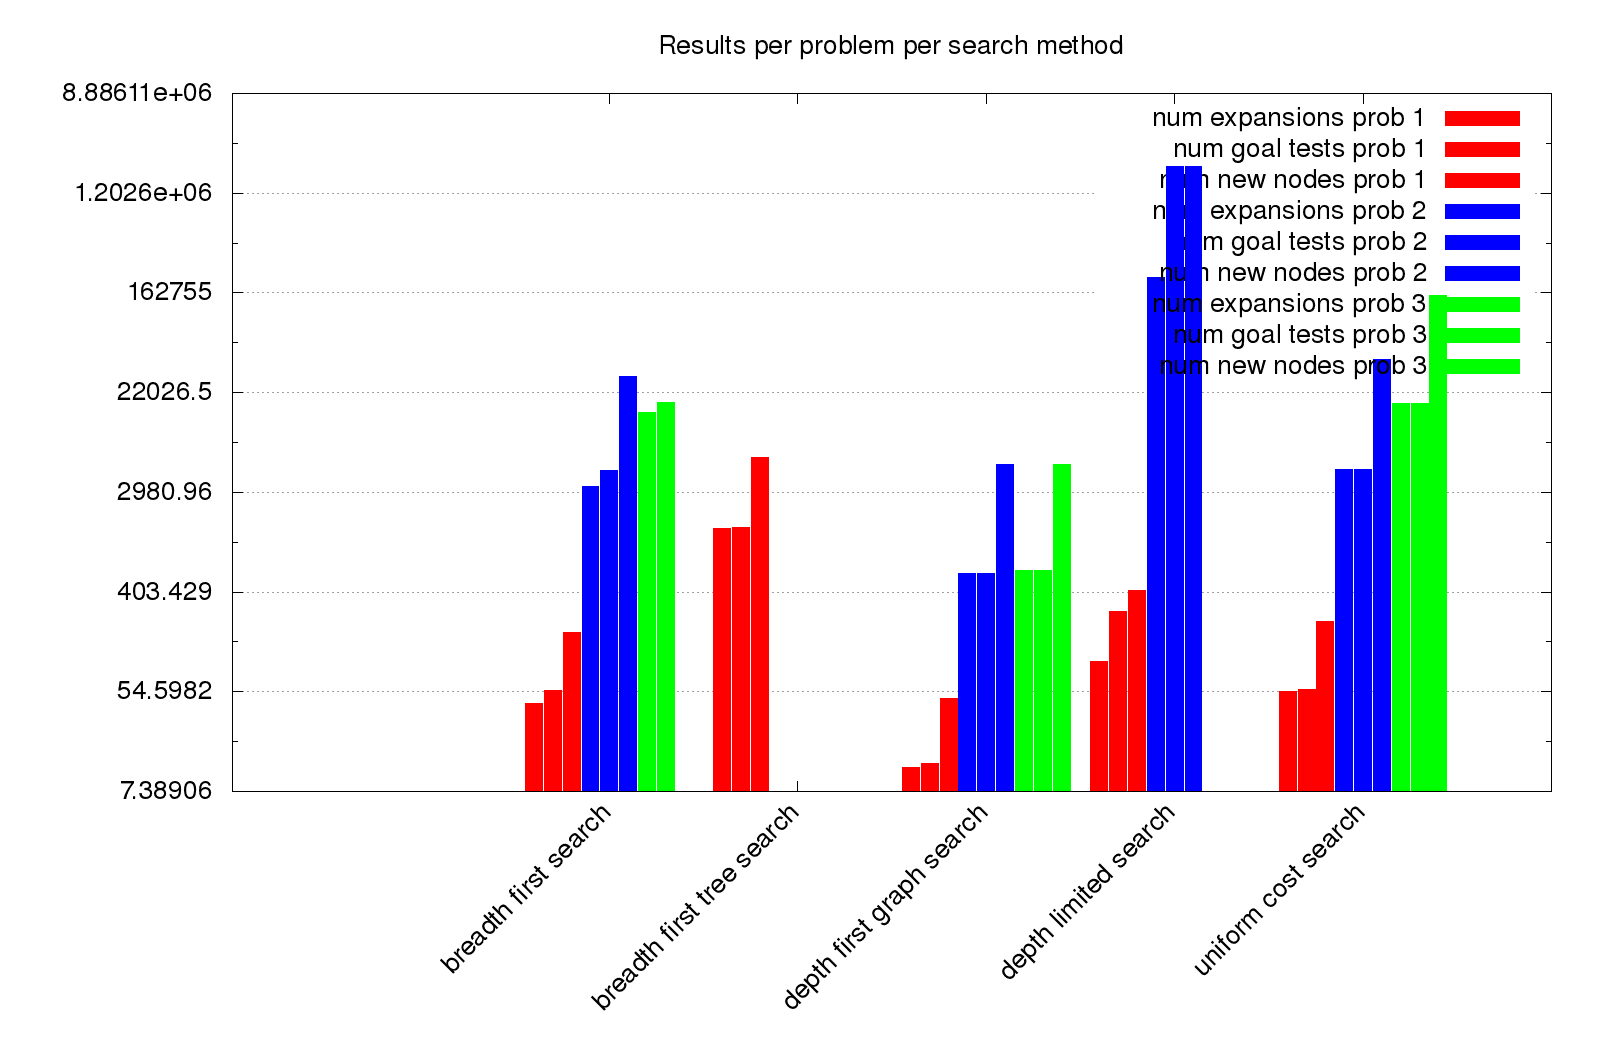
\includegraphics[scale=0.32]{results_summary.png}
	\caption{Results of each search method on each heuristic. The y axis is scaled to $log(e)$.
			 It should be noted that problems 2 and 3 were not solved by breadth first within reasonable time. and that problem 3 was not solved by depth limited in reasonable time.}
	\label{results}
\end{figure}



\subsection{Problem 1}

\subsection{Problem 2}

\subsection{Problem 3}



\end{document}
